\clearpage
%//==============================--@--==============================//%
%\vspace{-1em}
\subsection{P3 | Introdução de uma velocidade const. segundo a horizontal}
\label{subsec:P3}

A passagem de uma bola saltitante aliada a um movimento horizontal, entre duas superfícies de impacto distintas, sugere uma alteração ao \textit{jump map} (\textit{vide} \hyperref[sec:intro]{secção introdutória}), no que toca ao coeficiente de restituição aplicado na atualização da velocidade.
$$ 
    \begin{aligned}
         &\mspace{36mu}\textit{\underline{Jump}}\\[-0.7ex]
         &\underbrace{v_z := -\alpha_1 \cdot v_z}_{\text{Superfície 1}}
    \end{aligned}
    \;\xrightarrow[y = 10\text{ m}]{}\;
    \begin{aligned}
         &\mspace{36mu}\textit{\underline{Jump}}\\[-0.7ex]
         &\underbrace{v_z := -\alpha_2 \cdot v_z}_{\text{Superfície 2}}
    \end{aligned}
$$

\iffalse
\noindent Concatenando os \textit{jump maps} para as duas superfícies ao fim de $n$ e $k$ ressaltos obtemos:

$$
    v_z(t_{n+k+1}) = -\alpha_1^{n}\alpha_2^{k} \cdot v_z(t_1)
$$
\fi %rever mais tarde, adoro-te :3

\vspace{1em}
\noindent $\pmb{\rightarrow}$ \textit{\textbf{Velocidade Horizontal}}

\noindent A velocidade horizontal imposta à bola, que governa o seu deslocamento para a direita não sofre qualquer tipo de alteração nem dissipação de energia ao longo de toda a trajetória, já que a aplicação de forças na bola em movimento ocorre somente no eixo vertical, ortogonal à velocidade.
\\\\
A análise da \hyperref[fig:2Pav]{seguinte figura} evidência a diferença entre as perdas energéticas nas respetivas zonas de atenuação para cada impacto:

\begin{figure}[H]
    \centering
    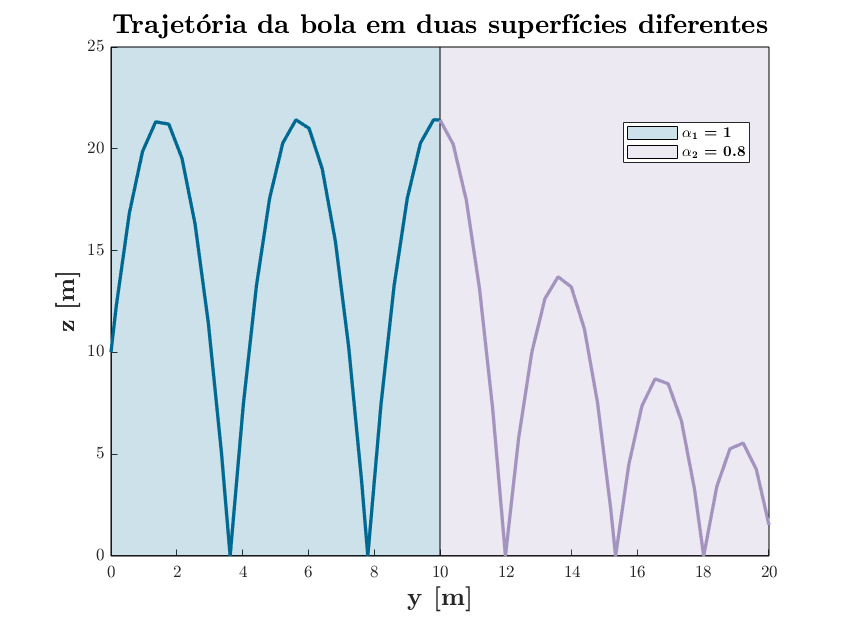
\includegraphics[width = 0.75\linewidth]{img/P3/P3-coefdif.png}
    \caption{Trajetória da bola em duas superfícies distintas com coeficientes de restituição $\alpha_1 = 1$ e $\alpha_2 = 0.8$ e para uma velocidade horizontal constante de $v_y = 1$ ms$^{-1}$ e $v_{z_0} = 15$ ms$^{-1}$.}
    \label{fig:2Pav}
\end{figure}

\noindent\textbf{\textit{$\rightarrow$ Observações}}
\vspace{-0.5em}
\begin{itemize}
    \item[$\blacktriangle$] A passagem da zona de colisão perfeitamente elástica ($\alpha_1 = 1$) para a de $\alpha_2 = 0.8$ verifica uma óbvia diminuição de altura máxima atingida. Como já referido, a atenuação imposta à velocidade vertical sofre uma alteração a partir de $y = 10$ m. Relembrando a discussão realizada na \hyperref[subsec:P1]{secção P1}, um menor coeficiente de restituição contribui para uma maior dissipação de energia a cada impacto, tal equaciona na já mencionada diminuição progressiva de altura comparativamente com a primeira zona de impacto (onde ocorre conservação total de energia $\rightarrow$ não ocorre atenuação da velocidade e consequentemente a altura atingida é sempre a mesma).
    
\end{itemize}
%//==============================--@--==============================//%